%\documentclass{../_combined/fcg-book}
\chapter{The Discrimination Game}

The previous chapter laid the perceptual groundwork 
for investigating conceptualisation and language 
communication. It proposed a set of mechanisms for segmenting a 
scene and extracting characteristics about each 
segment. The next task of the agent is to use these results
from the perceptual layer to categorize 
and hence conceptualise the
scene. For the time being, I will 
ignore the full complexity of natural
language meaning and focus only on the most 
simple type of conceptualisation one can
imagine, namely categories, which logicians refer 
to as unary predicates, as well as conjunctive 
combinations of categories. Words like "blue", "light" or
"square" name such categories. We not only need a way 
that the Talking Heads can use such categories to conceptualise
a scene based on visual perception, but we also need 
mechanisms that can explain how such categories might 
develop or be acquired by each agent autonomously and 
without supervised training. This is clearly an enormous
challenge and no known universally accepted solution 
exists to this problem.

Categorization has fascinated philosophers and scientists
since the beginning of thought, not only because it is one
of the most fundamental capabilities of the human mind, 
but also because the subject matter immediately raises 
some intriguing paradoxes and puzzles. First of all, 
we have already seen that there is an enormous 
gap between the symbolic world of objects and categories
and the subsymbolic world of analog sensory-motor signal streams. 
A particular sensory signal is highly context-dependent and
inherently noisy due to the partial
unreliability of sensors and their limited accuracy. 
Sensory processing, transformation, and scaling 
go some way to achieve perceptual constancy
but cognitive processes must clearly make up for
the fleeting erratic nature of reality. 
Here we are immediately confronted with a first paradox. 
Univocal categorization seems only possible when 
an interpretation of reality is within reach, for example
when there are strong expectations, possibly coming 
from language utterances. But this interpretation
depends itself on categorization. How can this apparent
causal circularity be broken? 

Furthermore, if it is already so difficult to map
categories on real world sensory data streams, how 
on earth can categories form and become stable? 
Young children appear to acquire perceptually 
grounded categories effortlessly and without systematic 
training. Psychologists have often observed the 
acquisition of distinctions
with very few clear example cases and no overt feedback. 
On the other hand, categories appear to 
some extent culture-specific and different 
individuals make more refined distinctions depending
on the sort of tasks they engage in. This is 
the case even in such a basic domain as colour categorization. 
Painters or textile designers make distinctions ordinary 
humans do not see and have developed a very extensive
repertoire of terms to talk about these distinctions. 
These observations highlight a second paradox: The 
effortless early acquisition of perceptual distinctions 
suggests that categories 
are innate. But the dependence on culture, individual
variation and specialisation suggest that categories
are learned. How can these two observations be reconciled? 

Then there is a third paradox, first suggested
by Jean-Jacques Rousseau. In order to communicate,
the speaker and the hearer need to share the building
blocks of the conceptualisations underlying their communication. 
If I say "the wine glass on the table", I expect 
the hearer to be able to recognise what objects are 
tables, when something is on the table or not on the table, and 
when something is a wine glass versus another kind 
of glass. But if every individual learns categories independently
and autonomously, how can they ever become shared? It is 
assumed that language helps in establishing a shared ontology within 
a language community but language itself depends on 
shared categories, so how can the whole system ever 
get off the ground; how can this chicken and egg situation
be broken?

I will begin this chapter by outlining the empiricist 
and rationalist positions, which have 
dominated much of the philosophical discussion on 
categorization and have indirectly influenced attempts 
to build artificial systems able to perform some form
of categorization. 
I will then propose an alternative {\it selectionist} approach
and study a categorization system based on it. It is 
shown that agents endowed with this system are able
to develop an adequate repertoire of categories for 
distinguishing objects in their environment and that 
this repertoire remains adaptive when important changes 
occur in the environment. This goes some way to 
resolve the paradoxes of meaning, but the story remains
incomplete. To explain how agents can share the same 
categories even if they develop their ontologies 
independently of each other, I will later argue for
a co-evolution of language and meaning. I will show
that when ontological development is coupled to lexical 
development, the two become co-ordinated with neither
a central co-ordinator nor prior design. 

\section{The paradoxes of meaning}

There are basically two philosophical doctrines that 
have tried to address the paradoxes of meaning. 
One doctrine is known as empiricism, the other one as 
rationalism.
Many philosophical texts are available introducing these
philosophical doctrines and their historical roots. 
The problem of the origins of language and meaning
was for example already a highly debated topic among philosophers in the 18th 
century, see for example \cite{Rousseau:1781}.
\newline
The debate between rationalism and empiricism
is still very much alive today and now based
on much more knowledge about what it means for 
something to be innate or what the limits are of
induction. See \cite{Elman:1998}
for the most recent arguments and counterarguments. Compared
to the full richness of human experience, I necessarily 
have had to adopt a very narrow view, focusing only on
basic perceptually grounded categories. More complex
categories related to human relationships, emotions, 
social organisation, beliefs, etc. will not be 
considered and it would be very difficult to do so 
with the methodology used here. See \cite{Varela:1991}
for a broader discussion.
\subsection{The empiricist's stance}

\is{empiricism}The empiricist tradition has a long and reputable
history. The first clear formulations emerged as a 
counterreaction to 17th century rationalism, with the work of 
Hume, Locke, and others. Empiricists
were inspired by the early success 
of the natural sciences, which had insisted on observing reality
as it is, through sensory experience and stepwise induction. 
The empiricist attitude has continued to dominate epistemology
in the 19th and 20th century. It was formulated by Bertrand
Russell in a doctrine called logical empiricism, and 
elaborated by generations of philosophers from Carnap to Quine
into rich logical frameworks and precise inductive methods. 
Empiricist explanations about categorization today very much
dominate the neurosciences. 

Empiricists argue that categories 
capture what is common or invariant between cases and that
neural networks in the brain
can detect this invariance. They also argue
that these commonalities can be learned
by progressively abstracting away from the details of specific
cases, even if there is a poor stimulus. 
A child sees many examples of red objects and
progressively grasps the abstract concept [RED] 
by retaining what is common to all of them. 
If categories are the result of a general 
inductive learning procedure, the areas of the brain
responsible for categorization do not have to be
specialised or pre-programmed for recognising 
specific categories. Empiricists therefore believe that 
they can take the 
form of general purpose networks that learn any kind 
of category by making abstraction from the examples 
supplied by the environment. Categories are therefore
not innate but learned. 

In recent decades, various designs for neural network models
have been proposed that reflect this empiricist stance.\footnote{
The first neural network models emerged in the 
fifties from the work of neurologists and computer 
scientists like Donald Hebb, McCullogh and Pitts, 
Rosenblatt, and others. There was a strong first wave of 
enthusiasm in the sixties, as illustrated for 
example in: \cite{Minsky:1968}. 
A second wave developed in the mid-eighties when 
new more powerful network architectures were discovered
that could handle intermediary representations and 
later on temporal structures (see the overview 
in \cite{Churchland:1992}. }
The input nodes of these networks receive data
from sensory channels of the sort discussed in the 
previous chapter. They are connected to higher
level nodes which use the data to decide whether
a category applies. The connections are weighted and 
a positive output signal is produced when 
the weighted sum of the inputs 
exceeds a certain threshold. Thus the networks
exhibit some of the flexibility, tolerance
to variation, and context-dependence seen in human
categorization. The weights and thresholds are 
learned by propagating back errors in categorization. 
If a node makes a positive identification when 
it should not have done so, the weights of the 
incoming connections are lowered and the threshold is
increased, so that it is less likely that the threshold
will be exceeded again for the same situation the next time around. 
Conversely, if the network makes a negative identification where
it should have made a positive one, the weights 
of the incoming connections are increased 
and the threshold lowered. It is known 
through mathematical proofs that such networks indeed
stabilise on reliable categorizations, if the 
environment remains sufficiently constant.\footnote{
This type of neural networks and some of its
main variants are discussed at length in the classical 
textbook by Rumelhart and McClelland \cite{Rumelhart:1986}.}
These inductive neural networks therefore
constitute ther first serious proposal for bridging the gap between
sensory signals and categories and for explaining the 
origins and acquisition of categories. 

\subsection{The rationalist's stance}

\is{rationalism}A radically different approach to categorization has been 
proposed by rationalists. 
The rationalist point of view had its first clear formulation 
in Plato's philosophy. A resurgence of rationalist ideas
took place in the 17th and beginning of the
18th century, particularly through the work of 
Descartes and Leibniz. More recently, in the second half of
the 20th century, a strong rationalist movement
emerged again, mainly under the influence of Noam
Chomsky. Today rationalist attitudes very much 
dominate linguistics and cognitive psychology. 

Early rationalists, like Descartes, were dualists, which
saw the mind and the body in totally different realms. 
In such a view, it becomes very difficult to scientifically investigate 
perceptually grounded categorization, and an explanation 
how the brain works seems more remote than ever. However, 
most contemporary rationalists (like empiricists)
now believe that categorization
is done by physical structures in the brain. Indeed, 
if certain parts of the brain are damaged, the capability 
to categorize disappears or is severely restricted and 
distorted, \cite{Deacon:1998}. 

Rationalists claim that categories 
exist {\it a priori} and therefore categorization comes from
within. They argue that humans have a repertoire of ideal universal
forms, which they project
onto reality. Reality itself is a weak, imperfect 
reflection of these forms, like the shadows of objects
on the wall of a cave. Because of this poverty of stimuli, 
categories (particularly the perceptually grounded
categories that are the focus of our attention in this 
book) are claimed to be unlearnable by induction and must
therefore be innate.\footnote{
Strong forms of innateness have been defended by 
\cite{Fodor:1983}
and many philosophers and linguists associated with the 
generative grammar paradigm. See the discussion in
\cite{Wierzbicka:1992}, particularly the introductory chapter. 
In artificial intelligence 
research, particularly the logic-oriented tradition, there
is often an implicit acceptance that basic categories 
are innate, but that derived categories (formulatable
in terms of more primitive concepts) can be learned
(see \cite{McCarthy:2008}). There are also 
large-scale efforts going on to build an ontology as 
rich as human ontologies, see the discussions around
Doug Lenat's CYC project in: \cite{Steels:1994}.}

\is{innate categories}This innateness hypothesis suggests that the brain comes
with `categorization organs', small neuronal circuits
capable of performing 
the mapping of some idealised universal form onto
reality. Consequently the human genome
must include a set of `concept genes' which regulate how each of 
these categorization organs should grow during 
development. Rationalists claim
that it is absurd to think of categories as being 
learned from example cases supplied by the environment, just 
as it is absurd to say that the hand learns to 
grow five fingers.

\subsection{Arguments for and against rationalism}

There is something to say both for a rationalist and 
for an empiricist approach, indeed otherwise so many
serious thinkers could not have believed fervently 
in one position or the other. Rationalists point to the 
fact that children acquire concepts
surprisingly quickly and apparently with very little stimuli
and that anthropological observations have 
shown that there are strong universal tendencies
for basic perceptually grounded categories, such as colour or 
space. However, more detailed observations show
that the acquisition of categories in children goes 
in fact very slowly. For example, concepts like cause-effect
and the correct use of the word "because", the proper
use of tenses, etc. all take years to develop. 
Adults keep acquiring
new categories through out their lifetime, which makes 
it difficult to maintain that they are part of the 
human genome. For example, 
airline pilots and sailors categorize the direction and 
strength of winds and the shapes and colours of clouds, 
so as to predict turbulences, future weather, or 
advantageous trajectories. There are
occasionally profound differences in how cultures conceptualise
reality. These differences do not seem to be innate because
everybody who has had sufficient exposure to the 
culture, preferably at an early age and therefore without too much 
preconception, can normally acquire them.\footnote{
Rationalists often argue that there is no other way 
to explain the child's rapid acquisition of concepts
but detailed psycholinguistic observations have shown that 
child language understanding (which is the 
clearest sign whether certain concepts have been acquired)
is often deceptive because 
non-verbal strategies may lead to appropriate answers
to adult questions and thus the appearance of 
understanding.}

Further objections against the innateness hypothesis have come from the camp 
of neurobiology. In lower animals, neural circuits have been identified which perform 
very specific categorizations of reality. For example, the 
frog is sensitive to objects of a particular
size moving in front of it at a particular speed, specifically the
kind of objects that constitute a potential 
source of food for the frog. The dedicated neuronal 
circuits performing this categorization have been 
shown to be innate and shared by all frogs. But higher 
animals and humans
exhibit an enormous plasticity, both in terms of the 
repertoire of categories they recognise and in terms of 
the actual brain structure.\footnote{
Evidence for the remarkable plasticity of the human 
brain is reviewed in \cite{Edelman:1987}and \cite{Elman:1998}. }

The difference between an animal
reacting to a limited set of environmental stimuli with 
a rigid neural apparatus and a cognitively endowed
human being is precisely the high degree of flexibility and 
adaptivity of the latter.
It is therefore not surprising that clear-cut 
`categorization organs' which have the same structure in 
all humans and are located at the same position in the 
brain have not been found. The microstructure of the
brain does not consist of
neatly separated organs and it therefore does not make 
sense to look for genes that regulate their maturation. 
Neurobiologists tell us that 
the brain appears more like an organically grown 
tissue rather than a delicately tuned machine laid
out by genetic programs. In contrast to insect brains or 
brains of lower animals, the mammalian brain is 
capable of regenerating itself to some extent after
damage, and brain tissue
from one higher order animal can be implanted in another
one, causing a resurgence of lost function, even if the 
source location of the transplant is different. 
For example, if tissue from the visual cortex is
implanted in the auditory cortex, it will 
regenerate and function as part of the auditory 
cortex. Pathways to the visual cortex can be
redirected to the auditory cortex, which will cause 
the auditory cortex to take on functions of visual processing. 

Even supposing that there is a strong genetic
determination of micro-level brain structure, there is 
still the question how the hundreds of thousands of concepts 
employed by adult human beings might have become 
included in the human genome. Saying that a perceptually 
grounded category is innate does not explain anything.
One has to show a plausible evolutionary history for 
the categories hypothesised to be innate and prove 
that the hypothesised concept genes can propagate sufficiently 
fast in the human population.\footnote{
See: \cite{Worden:1995}. 
This article argues, based on the genetic difference
between humans and other primates, that there are limits 
to genetic transmission of cognitive content, like 
categories or grammars. For discussions on the speed
of gene spreading compared to cultural evolution, 
see: \cite{Cavalli:1995}}

\subsection{Arguments for and against empiricism}

Empiricists have had considerable
success in coming up with inductive learning mechanisms. 
They have even been demonstrated on autonomous robots 
in direct interaction with the environment.\footnote{
Typical examples of this work can be found in the 
Proceedings of the Simulation of Adaptive Behavior 
conferences published by The MIT Press, Cambridge.}
At the same time, the learning mechanisms proposed so far turn out
to be very fragile.\footnote{
The weakness of traditional connectionist networks
with respect to speed and resilience
are discussed at length in \cite{Quartz:1997}.}
The human experimenter has to carefully 
set up the architecture of the network (the number of
nodes, the number of layers of nodes, and how they are
connected), tune the learning
parameters, and supply just the right set of test cases. 
Performance may degrade when too many cases are seen. 
Even worse, when new cases are supplied that require
a revision of categories already learned, a substantial
portion of the earlier cases must be resubmitted to 
retrain the network. All this contradicts
the robustness and open-ended extensibility
of human categorization. In addition, 
the learning mechanisms proposed have been
slow to consistently aquire categories. A large number of cases
are required and often 
cases must go through multiple iterations. Moreover 
any inductive method is a slave of
the data. A category will only become reliably recognised
when it is statistically significant. 

So there are questions both for a rationalist and an 
empiricist approach. If categories are innate how can
new categories, which are required when the environment
or the task settings change, form so quickly?
How can the genetic code store the vast repertoire 
of categories humans routinely 
employ, and how can we explain the diversity with which different
cultures approach reality? On the other hand, if every 
child independently acquires categories by learning, we 
must question how 
can they do so, given the poor quality of the examples 
they see. How is it that learning is so rapid? How can different
independent learners arrive at a repertoire of categories
that is sufficiently shared to make language communication
possible? How do we reconcile the apparent 
innate origins of perceptually 
grounded categories with their remarkable adaptedness to the 
changing needs and open-ended environments that the individual
effectively encounters? 

\section{Selectionism}

\is{selectionism}The difficulties encountered with the empiricist
{\it and} rationalist points of view make it worthwhile
to explore alternative solutions. The one I propose
and further explore in this book 
has been inspired by two key principles 
from biology. The first principle is
that of selectionism. It requires 
a growth process in the agents that generates possible 
structures, even in the absence of examples, and a pruning
process that removes those
that are irrelevant. The growth and pruning
process is assumed to be biologically given
but not the categories that result from it.  
The second principle that \is{interactionism}
I will adopt is interactionism, put forward by biologists 
to understand how genetic influences {\it and} environmental 
impact cooperate to shape an organism. Interactionism 
was first suggested by Piaget (originally a biologist)
to explain the growth of mental capacity in the child. 
His numerous experiments show a gradual progressive construction of 
increasingly more complex ways of categorising and 
conceptualising reality. The child encounters situations that 
can be assimilated, and thus cause entrenchment of
existing structures, as well 
as situations that cannot be handled and require 
the child to accomodate with new 
constructions or reorganisations.\footnote{
The work of Waddington is typical for the 
interactionist approach to development (see: \cite{Waddington:1975}). 
Such a view does not necessarily imply that there is 
a pre-determined course of development.
Piaget emphasised a progressive, dynamical view on 
development \cite{Piaget:1985}. 
His work arose prior to the detailed
computational modeling that is now common place in 
cognitive science and there is still an enormous 
work left to demonstrate operationalisations of these
insights. See for a more recent discussion of 
the issues \cite{Thelen:1994}.}

\subsection{Principles of selectionism}

Selectionism is a general means of explaining the origins of 
complexity. It requires: (1) a process that 
can generate a repertoire of possible solutions in a 
basically random fashion, (2) a process for preserving 
solutions so that there can be a gradual build up of 
more complex solutions, and (3) a 
selectionist force, which uses
feedback from the environment and influences preservation
so that adequate solutions are retained 
and others discarded.\footnote{
There are many excellent introductory 
accounts of selectionism. One of the best
known is: \cite{Dawkins:1995}. The 
recent application of selectionism to the automatic
derivation of computer programs clearly demonstrates
how general the principle is. See: \cite{Goldberg:1989} and \cite{Koza:1997}. 
The principle has now even been applied to 
the development of computational hardware. See: \cite{Sipper:1998}}

In the case of the Darwinian explanation for the 
evolution of species, a solution is an organism 
capable of surviving in a given environment. Types 
of organisms are preserved in the genetic material as 
it is copied from one generation to the next. 
Variations are produced due to errors in gene copying, 
mutations, gene insertion, etc. The feedback comes
from the natural environment. Organisms that do not flourish are
less successful in reproduction so that their
genetic material and hence the organisms 
this material generates are less likely to be preserved. 
Selectionism contrasts with Lamarckian instructionism, which 
claims that the organism transmits its adaptations 
and what it has learned during its life time to 
its offspring. \is{instructionism}

From the viewpoint of instructionism, the
neck of a giraffe is so long because at some point
giraffes with shorter necks often stretched
their necks. This was transmitted
to the offspring which got born with slightly longer necks.
They also stretched their necks further, 
and so on. In a selectionist framework, it is assumed
that the natural variation in the population 
is exploited. Some giraffes have longer necks than 
others, and if this gives an advantage 
their genes proliferate. Within the population born with the 
new gene distribution there are still variations and 
once again those with a longer neck proliferate, and so on. 
Instructionist processes build further upon acquired characteristics. 
There is progressive learning from one 
generation to the next. Selectionism assumes natural 
variation and progressive dominance of fitter variants, with 
neither learning nor transmission of acquired characteristics. 
Selectionism can make sudden jumps and therefore has the 
potential to go much faster than the transmission of acquired
characteristics. 

In the case of the immune system, a `solution' is an 
antibody capable of combatting intruders foreign to the 
organism. Here again an instructionist approach can 
be envisioned and was believed for a long time to be 
the case. For this belief to be true would mean that
the immune system somehow `learns'
the appropriate response
and then preserves that response. The selectionist viewpoint
of the immune system argues instead that it
generates autonomously 
a very large repertoire of possible antibody responses. 
When a foreign body invades, the response 
is already 
there, it is simply a case
of amplification, \cite{Varela:1988}. 

\subsection{Selectionist cognitive systems}

The Talking Heads experiment explores the same line of thinking, 
both to the acquisition of categories, and later
(in volume 2) to the acquisition of more complex meaning 
and even grammar. It implies
that there is no learning taking place in the empiricist sense 
of induction from a series of examples, but that instead 
three processes are active: 
(1) a process whereby structures capable to categorize
reality are generated in a basically random fashion, 
(2) a process to preserve these structures and build 
further upon them to enable a steady increase in 
complexity, and (3) a selectionist force which
prunes away those structures that were irrelevant and 
retains the ones that are successful and needed. 

As I will expand upon in more detail in this 
chapter, categorization
can be carried out by discrimination trees where the 
nodes in the tree filter objects depending on whether they 
fall within a sensory region or not. I will show that
the discrimination trees grow in a more or
less random fashion and 
those parts of the tree that are irrelevant get pruned. 
The selectionist feedback comes from the games in which 
the agent participates. Distinctions that are effective
in discriminating the topic from the other objects in 
the context and have been successfully lexicalised, 
are maintained in the lexicon of the
community, others are discarded.

When there is a high failure rate, the discrimination trees 
should expand, in the same way that the immune system gets 
stimulated (but does not strictly speaking
learn) when the organism is
invaded or genetic variation increases in periods
of stress on a species. When there is a high
success rate, some pruning
might be possible. The growth and pruning dynamics creates an 
ecology of distinctions which is constantly 
adapting itself to the situations and tasks 
the agent encounters, without any innate {\it a priori}
categories and without any inductive learning. 

\subsection{The tree metaphor}

The growth of a tree or plant is a good 
metaphor to visualise this selectionist approach. 
The shape of a tree appears well adapted to 
its environment. Typically there are more branches and leaves 
where there is more sunlight. The height of
the tree reflects the competition of neighbouring trees
or the height of surrounding buildings. The overall shape reflects
the shape of surrounding walls or other trees. 
It is obvious that a tree
does not come with "shape genes" that determine
exactly which shape the tree will have in a particular 
setting. Nor does it come with sophisticated sensors
and a brain inductively learning about the environment
so as to decide on which branch the next leaf should grow. 
Instead the tree grows in all directions following
a steady, usually quite regular growth pattern. A tree
standing alone in a landscape exhibits a beautiful 
balanced shape, expanding in all directions, but when the 
growth is constrained, the tree reflects these constraints. 
The branches and leaves that catch more sunlight receive more resources 
to flourish and develop further, whereas those 
pointing towards an area with no sunlight are stifled in 
their growth and may die altogether.  

Given that the brain is a living tissue, it is possible 
to imagine a similar growth process in the brain.\footnote{
Several neurobiologists have presented 
suggestions and evidence in this direction. See 
particularly \cite{Edelman:1987} and \cite{Changeux:1997}.}
Neural networks implementing discrimination trees could be expanding
in all directions, just as other
tissue forms. The overall growth dynamics is 
genetically determined but neutral with respect to 
the repertoire needed in a certain environment. 
The shape of the discrimination trees in a particular 
individual is due to the kinds of sensory 
data that have been produced in his interactions with
the environment {\it and} their use and success
in other cognitive processes such as language
communication. The
users of the discrimination trees and the environment act
as selectionist forces molding the spontaneously forming 
repertoires.

Note that selectionism is NOT applied at 
the level of a species as in biological evolution but 
at the level of the cognitive structures in each individual
as he or she develops and adapts during his or her life 
time. The parallel exploration and the competition of 
alternative ways to categorize reality take 
place in a single individual interacting with the environment
and therefore are very rapid.

\subsection{Deriving new sensory channels}

Obviously the sensory channels are a critical 
part of the categorization process. When the sensory data is 
not available, it is simply not possible to develop 
discrimination trees along a particular sensory dimension. 
This raises the question as to where the sensory channels
themselves may come from. 
The most basic raw data is directly supplied by
the sensors themselves and is thus innately given. But 
processes calculating the values on 
the more complex channels must somehow form under the 
influence of the environment, and they are
thus potentially partly influenced by language. 

Here again both an inductive and a selectionist approach
can be envisioned. In an inductive approach, a learning
process, such as embodied by a connectionist network, 
is fed with a series of examples of situations 
exhibiting particular characteristics, and the network 
becomes sensitive to the characteristics of these
situations. Several concrete examples of such a 
learning process have already been studied 
using the neural network techniques mentioned earlier.\footnote{
Examples are discussed in: \cite{Linsker:1990}.} 

In a selectionist approach, a repertoire of primitive operations
is given, presumably implemented by the 
basic biochemistry of the neural systems, and there are
ways to combine these operations into more complex
`visual programs'. Those
programs yielding an outcome which
is afterwards used successfully in categorization are 
retained and the others discarded, thus establishing 
a co-evolution between a repertoire of sensory channels
and a repertoire of 
categories. We have already done some successful experiments 
in this direction (\cite{Dejong:1999}) 
but this theme will not be pursued further here as a full discussion 
would be too much a digression from the main line
of investigation. For the remainder of this book,
the sensory channels will be pre-programmed, 
although it is still up to the selectionist 
categorization process to discover which ones are useful
in the environments presented to the agents and which 
ones are not. 

\subsection{Comparing approaches}

A selectionist approach is different from 
both the rationalist {\it and} empiricist points of view.
In contrast with rationalism, it is not assumed that categories are
universal and {\it a priori} shared. Categories are not innate. 
In contrast with empiricism, it is not assumed that 
categories are derived by induction from a large 
set of cases. Categories are not learned. What is 
claimed to be innate is a general purpose growth and pruning
dynamics which could be realised by the biochemistry of
neural cells. The growth process may generate many categories 
which may turn out to 
be useless, but eventually it settles on a repertoire
which is adequate for the environment in which the 
individual finds itself. 

A selectionist approach to category formation has some 
characteristics that make it look like categories are 
innate. Categories may form in an individual
without having ever seen one single example. They
appear to pop up from nowhere, but this does not 
mean that genes determining this particular category have 
to be innate. They are the result of a random growth process
which has simply generated these possibilities. 
Alternatively, a selectionist process has some characteristics
that make it look like categories have been learned.
The individual ends up with a repertoire
which is adapted to 
the environments and tasks that are indeed encountered, and 
this ontology keeps evolving to remain adequate when 
the environment changes or new tasks are encountered. 
Because the selectionist approach has characteristics
of innateness as well as learning, it is capable of helping
resolve the 
paradoxes of the origins of categories discussed in the 
beginning of this chapter.  
It explains adaptivity without learning and fast 
development, even with a weak stimulus, but without innateness. 

All of this sounds intriguing and brings in a refreshingly new 
point of view, but does it really work? Can we 
invent the required growth and pruning dynamics and 
identify the appropriate selectionist feedback loop? 
The remainder of this chapter focuses on this question. 

\section{Discrimination trees}

First I will introduce structures that can perform
categorization. The next section shows how these
structures may autonomously originate in an agent
interacting with the environment. \cite{discrimination trees}

\subsection{Making distinctions}

Empiricists start from the idea that categories 
capture what is common
between objects. Thus [RED] is supposed to capture 
what is common or similar to all 
red objects. Hence in theories of 
(formal) semantics, the meaning of a predicate is 
equated with the set of all things that 
belong to the class it delineates. 
But we can also turn things around. We can 
view a category as a way to capture what is {\it different} 
between objects. For example, the distinction between 
[LEFT] and [RIGHT] is based on the horizontal position (HPOS)
of an object with respect to the viewer. 
The distinction is imposed on the scene (as long as 
it is compatible) instead of 
recognised. This may seem a subtle difference, but it
has profound consequences, particularly for acquiring
categories.

Consider the category [LARGE]. What do all large 
objects have in common? At first sight very little. 
Almost any physical object can be called large in 
one context or another. 
It is going to be very difficult for a learning agent
to determine some commonality, even if given thousands 
of examples of large objects. In the beginning, the agent
might be confused by commonalities in 
colour or position or shape. 
Only with some luck, will the learning algorithm
start to zoom in on size. 
This is what makes inductive learning so slow and 
why it is criticised, rightfully, by rationalists. 
In fact, searching for commonality hardly makes sense for
many categories. [LARGE] is only meaningful in
opposition to [SMALL], [LEFT] only makes sense
in opposition to [RIGHT]. Often categorization
is relative to the context (a block which is large when surrounded
by smaller blocks may be categorized as
small when surrounded by larger
blocks) and occasionally it is relative to the objects themselves
(a large mouse is always categorized as
much smaller than a small elephant). 

Few people would disagree that [LARGE] and [SMALL] are
distinctions imposed on reality as opposed to intrinsic
properties of classes of objects, but what about colour? Is it
not an example where a category is absolute? We have 
already seen in the previous chapter that this is not 
the case. The colour reflection depends strongly on the 
surface reflection and thus on the light conditions and
light sources in the environment. What should objectively 
appear blue when measuring the wavelength might actually 
appear green and vice-versa. Colour is {\it not}
an intrinsic property but is actively mapped onto reality
in a context-sensitive way.\footnote{
As mentioned earlier, see the discussion about colour 
in \cite{Varela:1991}.}
This does not mean of course that categorization does not make use of sensory
data. On the contrary, without sensory data, categorization
would be entirely impossible. 

Once categories are available, they can be 
used for much more than making distinctions. For example, 
if an agent has the distinction between [LARGE] and [SMALL],
he can use it to group the objects in a scene into two
subsets: those that are large and those that are small. 
So in this case, the categories are used to group 
objects based on a characteristic they have in common, 
namely being large and being small. My main argument here is that 
categories form driven by discrimination tasks,
afterwards they can be used for many other 
semantic processes, including classification. 

\subsection{Categorizers}

I will refer to the process capable of making a distinction as
a {\it categorizer}. \cite{categorizer} It operates on the output of 
a sensory channel and decides whether a category or its opponent
is valid. A categorizer keeps track of its success 
by maintaining an internal counter. 
Consider for example the category [LARGE] which 
operates on the output of the AREA-channel. This channel 
contains a scaled value 
between 0.0 and 1.0 for the area of a segment. A distinction 
can therefore be 
made simply by dividing the set of possible values in two
halves: those whose area is between
0.0 and 0.5 and those whose area is between 0.5 and
1.0, giving us two categories, [SMALL] and [LARGE]. When 
the agent needs to categorize an object, he checks in which
region an object's area falls. If it is between 0.0 and 0.5, the
category is [SMALL], if it is greater than 0.5 the category
is [LARGE]. 

It is clearly possible to refine each 
category $c$ by introducing categorizers that 
further divide the region of possible values of $c$ into 
smaller subregions. For example, the category [SMALL] which 
is applicable if the area is between 0.0 and 0.5, can be refined 
by introducing two more specific categorizers: one responding
to a region between 0.0 and 
0.25 for [VERY-SMALL] and another one for a region
between 0.25 and 0.5 for [MEDIUM-SMALL]. The total set of
distinctions using values of the same sensory channel
can be organised in a discrimination tree (\figref{trees}). 
\begin{figure}[htbp]
  \centerline{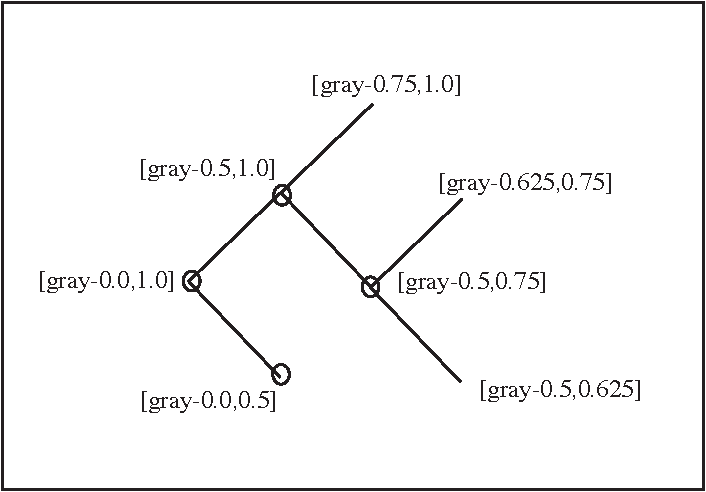
\includegraphics[width=.65\textwidth]{chap4/figs/tree}}
\caption{\label{trees} A discrimination tree contains
a set of categorizers which categorize by checking whether
a sensory value falls in the region of one category or 
not. The discrimination tree shown operates on
values on the GRAY channel.}
\end{figure}

As mentioned earlier, I will label categories
by using the sensory channel from which a category operates, 
followed by the minimum and maximum values of the region
carved out by the category. For example, 
[AREA 0.0-0.25] carves out the region [0.0,0.25] of the 
area channel. When it must be emphasised that 
a category belongs to a particular agent, for 
example {\bf a1}, I will write [AREA 0.0-0.25]$_{\bf a1}$. 

Conjunctive combinations of categories also have
dedicated categorizers which are linked to 
the categorizers of their components (see 
\figref{disnet}). A conjunctive combination 
often yields a more efficient way to pick out 
the topic compared to a single, possibly very fine-grained
distinction. For example, it might be that 
[AREA 0.0-0.25] {\it and} [GRAY 0.5-1.0]
together are distinctive but none of the two on their
own is. Other logical combinations are equally of interest
but I will restrict my attention to conjunctive 
combinations. Conjunctive combinations of categories 
will be written between curly brackets (\{,\}) as in 
\{[AREA 0.0-0.25] [GRAY 0.5-1.0]\}. 
\begin{figure}[htbp]
  \centerline{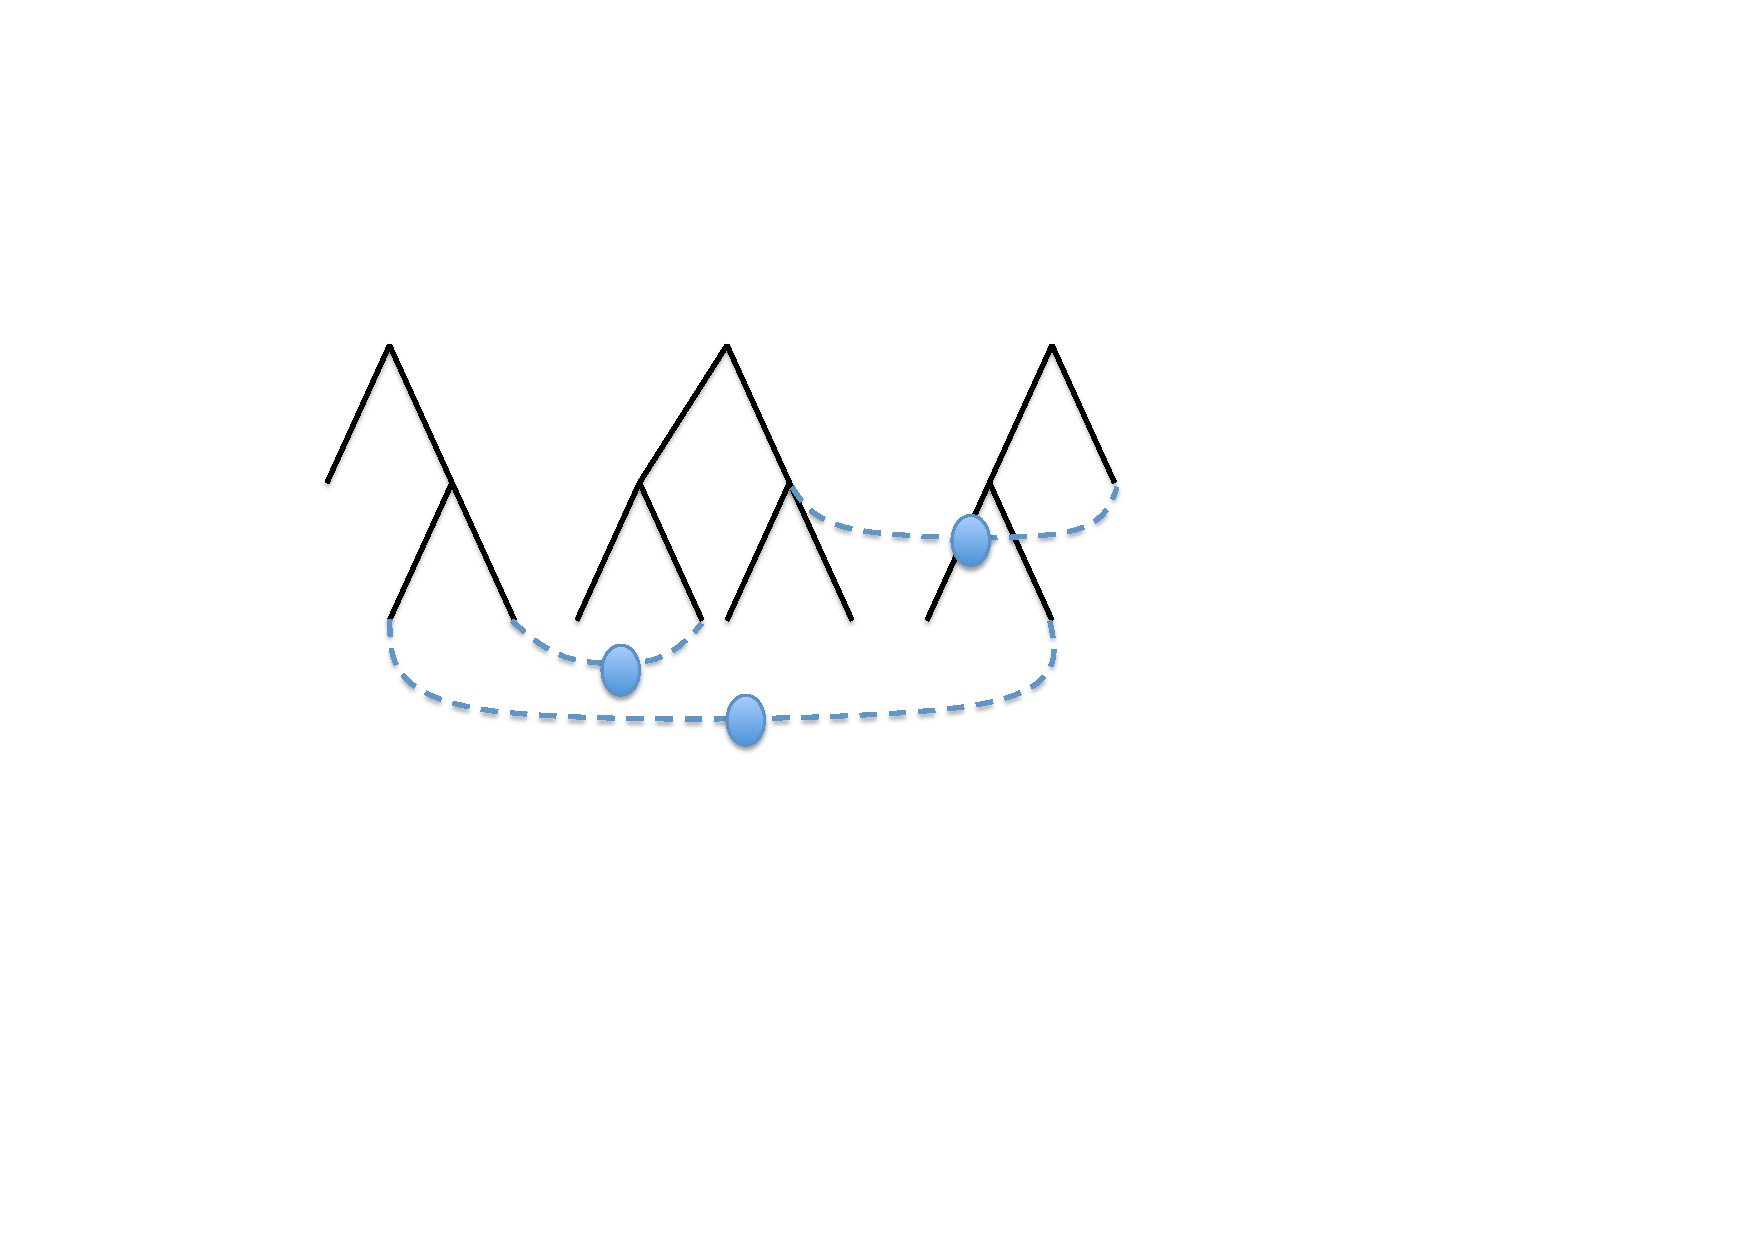
\includegraphics[width=.65\textwidth]{chap4/figs/disnet}}
\caption{\label{disnet} More complex categorizers
(shown as circles) are formed from the combination
of primitive categorizers.}
\end{figure}

\subsection{The discrimination game} 

\is{Discrimination Game}Here is a game, which I call the discrimination game, which is useful 
to study categorization in 
a systematic way.\footnote{
The discrimination game model together with the 
discrimination trees and its growth dynamics 
was presented for the first time in \cite{Steels:1996}
Based on this paper a new implementation of
single category discrimination was implemented by Angus McIntyre 
within the BABEL environment. Later on, Joris Van Looveren
re-implemented the use of conjunctive combinations.}
The game is played by a single agent, randomly 
drawn from a population of agents, and 
is equivalent to the conceptualisation phase of 
the guessing game. The agent perceives the scene and 
chooses a topic from the possible objects segmented in the
scene. He then uses his discrimination trees, as developed so
far, to come up with a category or a conjunction
of categories that is valid for the topic, but not for any
other object in the context. The discrimination game succeeds if 
the agent has found distinctive categories, otherwise the game
fails. When the game succeeds, the success counter
of the categorizers involved go up. 
\begin{figure}[htbp]
  \centerline{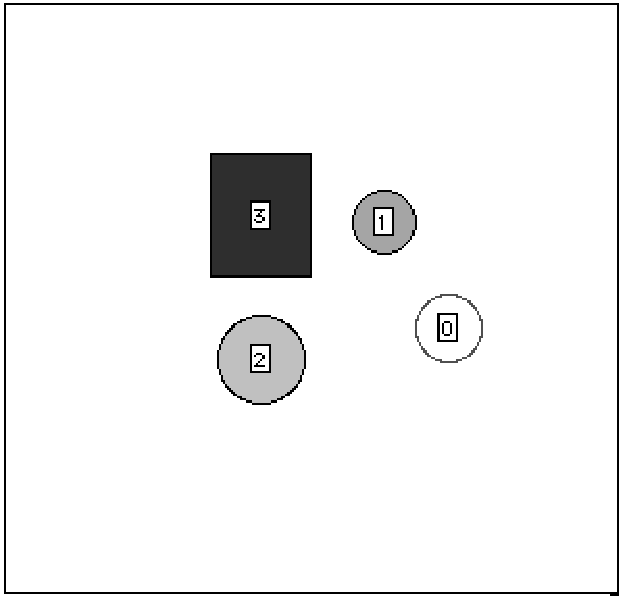
\includegraphics[width=.40\textwidth]{chap4/figs/game5}}
\caption{\footnotesize \label{geom} A computer generated scene 
from the GEOM world.}
\end{figure}

I will now develop some concrete examples, which imply
that I make choices for the kinds of sensory channels
and scenes that the agents use. 
I will first use scenes from the GEOM world as in 
\figref{geom} and later real world scenes captured
with a Talking Heads camera. 

Consider the scene in \figref{geom}. Assuming that the agent
already has a well-developed set of categories, he could use 
the category [GRAY-0.75,1.0] (very dark) to distinguish 
shape 3 from the others. On the other hand, if shape 2 is 
chosen as topic, the grayscale will not be enough because
shape 2 has the same grayscale as shape 1. Maybe a 
combination of categories can be chosen, like [VPOS 0.0-05]
(lower), and [HPOS 0.0-0.5] (left). Indeed shape 2
is lower in the scene, as opposed to
shape 1 and shape 3, and it is more to the left compared 
to shape 0 and 2.

\subsection{The Pachinko machine}

\is{Pachinko machine}Any visitor to Japan sooner or later comes across a 
Pachinko hall where eager players sit before a 
machine in which a metal ball, inserted at the top, 
falls through a series of gates until it falls in 
a winning or a losing bin. These games are
a possible metaphor to visualise the categorization process
based on discrimination trees. 

Imagine that for each object in
the scene and for each sensory channel, there is a ball
containing the value for that object on that channel. It
is introduced in the top categorizer of the 
discrimination tree associated with that channel. 
For example, suppose that there are three
objects in the scene: $O1$, $O2$, and $O3$, 
with gray-scale values 0.6, 0.4, and 0.9 respectively. 
We can therefore imagine three balls labeled with these datavalues
which are input to the top categorizer of the 
GRAY discrimination tree (\figref{balls}). 
A categorizer divides the balls in two bins, 
those that fall in the range of 
one category and those that fall into the range of the other
category. In this case, the left bin contains \{$O2$\} 
(category [GRAY 0.0-0.5]) 
and the right bin \{$O1$, $O3$\} (category [GRAY 0.5-1.0]). 
\begin{figure}[htbp]
  \centerline{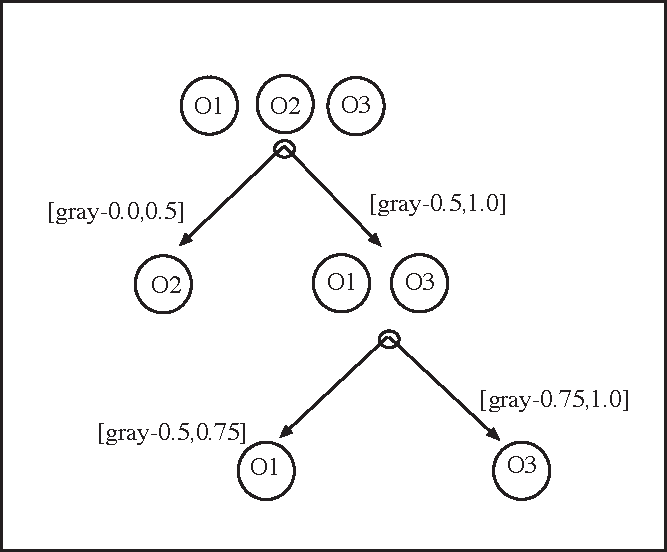
\includegraphics[width=.65\textwidth]{chap4/figs/balls}}
\caption{\footnotesize \label{balls} Balls containing
the data value for the different objects
$O1$, $O2$, $O3$ in the scene. $O1$ is the topic.
$O1$ has the value 0.6 on the GRAY-channel, $O2$ has
0.4 and $O3$ 0.9.} 
\end{figure}

A distinctive category is found when the ball of the 
topic is the only one left in one of the bins. 
If the topic is $O1$, then this is not yet the 
case, because it is together with $O3$ in the 
bin of [GRAY 0.5-1.0]. However when the next categorizer
is exercised, it splits the set \{$O1$, $O3$\} 
into two subsets: \{$O1$\} for [GRAY 0.5-0.75]
and \{$O3$\} for [GRAY-0.75,1.0]. 
[GRAY 0.5-0.75] is a discriminating category because only 
$O1$ is left in its bin. 

Balls thus trickle down from the top to the bottom of 
a discrimination tree, like in the Pachinko game or 
a lottery machine. The trickling down process can stop as
soon as a distinctive category is found because finer grained 
distinctions are not necessary. 

\subsection{Competition between categories}

A realistic agent has hundreds of sensory
channels, and humans probably have tens of thousands
of them, probably grouped with respect to the domains
to which they apply.\footnote{
This is strongly suggested by psychological 
data on the presence of conceptual spaces in human 
categorization. See \cite{Gardenfors:1999}.} There are discrimination trees
for each of 
these channels or for combinations of them, and 
each can possibly yield a distinctive
category. The categorization process can therefore be
envisioned like a huge Pachinko hall, in which
balls are trickling down in parallel in hundreds or 
thousands of machines. It is highly 
likely that more than one solution is found
when there are a lot of trees, particularly 
if combinations of categories are allowed as well. 
So, an additional competitive process must 
take place to rank categories even 
though multiple solutions are offered to subsequent
verbalisation processes. We see therefore the same
characteristics as for the perceptual layer, and thus
the `sieve architecture' also 
applies for the conceptual layer (\figref{f:sieve}). 
 
There are many possible criteria for preferring 
one category over another, equally distinctive one. 
The first is based on 
simplicity. A single category is less complex than 
a combination of categories, and a more abstract category 
is preferred over a more specific one. 
The second criterion is based on success in earlier games. 
Each categorizer monitors how many
times it was used and how many times
it was successful, i.e. how many times it could distinguish
the topic and participate in a successful language game. 
Another criterion, that I will bring in later 
once I have introduced the lexical layer, refers to 
success of the lexicalisations of the category. The agent 
will prefer categories where it is known that there is
a well-accepted way to express it. 
When ranking categories, these criteria are combined
and the best ones enter with the most force in the 
lexicalisation layer. 

Notice the hidden positive feedback effect\is{positive feedback} between success
and use: A categorizer which has already achieved
a higher score wins the competition, everything else being
equal, causing its score to increase even more. 
This way a consistent behavior emerges where the 
same category tends to be used in the same circumstances, 
similar to the way a walking path sometimes 
emerges for crossing a patch of grass between buildings. 
Initially many paths are possible, but once one path 
is used a bit more than others, it gets used more and 
more, as people reuse a path they perceive to be
there. I will show later (chapter 6) that this entrenchment of 
a particular solution by a positive feedback loop can 
be exploited through the structural coupling between 
the ontology (the set of categories) and the lexicon
(the set of form-meaning pairs verbalising categories), 
so that they become co-ordinated without a central 
co-ordinator.\footnote{
I adopt here other general principles of complex
systems. The notion of structural coupling has been 
introduced by \cite{Maturana:1992} and is 
now widely used to explain various forms of 
biological co-ordination.}

\subsection{Variations on discrimination}

There are obviously many variations on categorization
that could be imagined. For example, a categorizer
could make use of focal points instead of regions. A focal 
point is a single significant data value of a sensory channel.
The categorizer then has to compute the distance 
between the value for a segment and the focal point 
of each possible category. The category 
whose focal point is closest to the sensory value
of a segment applies. This implements a `prototype-like'
approach to categorization which has been argued to 
be more realistic with respect to human categorization.\footnote{
See \cite{Varela:1991} and \cite{Taylor:1989}.}
For example, humans typically label light
at 482 nanometer as the most typical blue, so that a given object
reflecting light at or near this point is categorized
as [BLUE]. Categories based on focal points are 
interesting and have clear advantages 
but I will stick nevertheless in the first instance 
to binary discrimination trees operating on single sensory 
channels to simplify the explanations
and to analyse better what is going on. 

Still another way to categorize reality is by imposing 
an order on the segments based on their values for 
a particular sensory channel. For example, we can 
order the segments based on the HPOS channel (i.e. 
from left to right) and then introduce relational categories
like `left of one segment in the series', or `the left-most object'. 
Similarly we can order the segments based on the 
HEIGHT channel (i.e. in terms of their size) and then 
have categories that select the smallest (i.e. the 
first segment in this ordering), or those greater than 
some other one. 

Of course, I am well aware that this categorization 
process captures only the most basic way of generating
meaning. Human beings make extended use of metaphor, 
analogy, metonymy, and other processes that adapt 
conceptual structures from one domain to another one.\footnote{
See: \cite{Johnson:1987}.}
But before we can study such processes we must understand
how basic perceptually grounded categories can 
originate. 
 
\subsection{The Discrimination Game in action}

Let us now look at some example 
games for an agent {\bf a1} taken from simulations
using computer generated
scenes from the GEOM world and showing the internal
structures generated as well as the reports from the commentator. 
At first I will not take saliency nor 
context-scaling into account. The first game
(game 8) fails. It takes place near the very beginning 
when {\bf a1} has practically 
no repertoire of distinctions yet. The scene and the 
discrimination trees available so far are shown in Figure 
\ref{scene2}. The object labeled 0 is the
topic. Only two channels have top level
categorizers: HEIGHT and WIDTH. 
The data on these channels for the scene in Figure
\ref{scene2} are shown in \tabref{tab:t-game8}. 
\begin{table}
\begin{center}
\begin{tabular}{| l | l | l |} \hline
{\it Object} & {\it HEIGHT} & {\it WIDTH} \\ \hline
0 (square) & 0.413 & 0.317  \\ \hline
1 (circle) & 0.410 & 0.410 \\ \hline
2 (square) & 0.163 & 0.163 \\ \hline
\end{tabular}
\caption{\label{tab:t-game8} Sensory data for the scene in \figref{scene2}.}
\end{center}
\end{table}

HEIGHT and WIDTH have been scaled with respect to the 
minimum and maximum height and width of a 
figure (sensor-scaling) but no context-scaling has 
been performed. 
\begin{figure}[htbp]
  \centerline{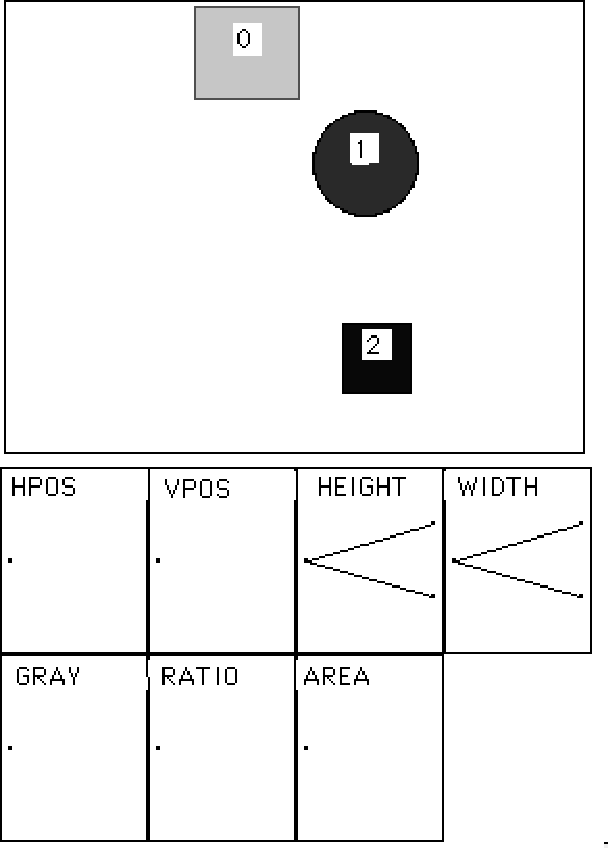
\includegraphics[width=.40\textwidth]{chap4/figs/scene8}}
\caption{\label{scene2} Top: The scene used in game 8. 
Shape 0 is the topic. Bottom: The discrimination trees available
for this game.}
\end{figure}
The game is reported by the commentator as follows: 
\begin{verbatim}
Game 8
 a1 segments the context in 3 objects: 
    square-0, circle-1, square-2
 a1 chooses square-0 as the topic
 The discrimination game fails
\end{verbatim}
The game fails because for the two sensory channels 
for which there are discrimination trees, the values 
of the segments are all within the lower range and so 
no distinctive category or category set could be found. 
This failure stimulates
the discrimination network to expand, but any node, 
including a top node of some of the other sensory channels 
can be chosen for further expansion. 

\begin{figure}[htbp]
  \centerline{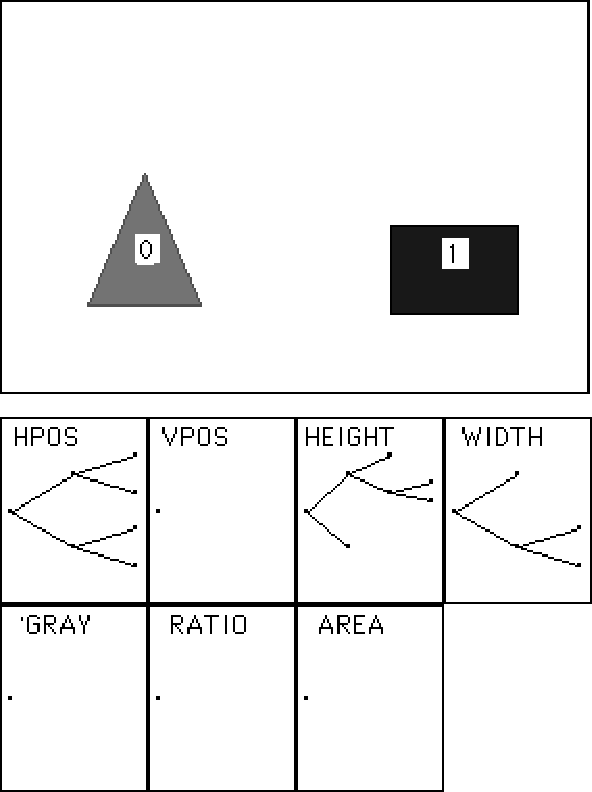
\includegraphics[width=.40\textwidth]{chap4/figs/scene22}}
\caption{\label{scene3} Top: The scene used in game 22. 
Bottom: The discrimination trees available to the
agent.}
\end{figure}
The next example shows a game (game 22) based on the scene 
in \figref{scene3}. The topic is the triangle, shape 0. 
The discrimination trees for 
HEIGHT and WIDTH have already more than one level and 
a discrimination tree for HPOS has developed.
The relevant sensor-scaled data for these three sensory
channels is shown in \tabref{tab:t-game22}. 
\begin{table}
\begin{center}
\begin{tabular}{| l | l | l | l |} \hline
{\it Object} & {\it HPOS} & {\it WIDTH} & {\it HEIGHT} \\ \hline
0 (triangle) & 0.167 & 0.437 & 0.573  \\ \hline
1 (rectangle) & 0.789 & 0.563 & 0.287 \\ \hline 
\end{tabular}
\caption{\label{tab:t-game22} Sensory data for the scene shown in \figref{scene3}.}
\end{center}
\end{table}

The scene is very simple so there are several possible
solutions: The triangle is more to the left, it is less wide 
and taller. Each of these possibilities is discovered
and their score (purely based on past performance) is 
looked up. The game is reported by the commentator
as follows: 
\begin{verbatim}
Game 22
 a1 segments the scene in 2 objects:  
   triangle-0, rectangle-1
 a1 chooses triangle-0 as the topic 
 a1 categorizes the topic as [HPOS 0.0-0.5] (score 0.57), 
   [HEIGHT 0.5-1.0] (score 0.09), or 
   [WIDTH 0.0-0.5] (score 0.0) 
 The discrimination game succeeds
\end{verbatim}

\subsection{The importance of scaling and saliency}

The example of game 22 shows at once why context-scaling 
and saliency is important. When we inspect the scene in 
\figref{scene3}, we do not quite see so clearly 
that the triangle is less wide than the square, so why
is [WIDTH 0.0-0.5] 
nevertheless considered? Examination of the data shows
that the WIDTH values, 0.437 for the triangle
and 0.563 for the square, are very close 
to each other, but just by luck fall within 
the two regions carved out by the WIDTH discrimination
tree. On the other hand, the values on the HPOS channel 
are much further apart and so they are preferred. 

As we have seen in the previous chapter, 
saliency is the smallest of the absolute values     
of the distance between the topic and any
other object. It gives us an indication why 
a certain sensory channel should be preferred
over another. For the scene in game 22, the saliency for each channel with 
respect to the triangle is as in \tabref{tab:t-game22-sal}: 
\begin{table}
\begin{center}
\begin{tabular}{| l | l | l |} \hline
{\it HPOS} & {\it WIDTH} & {\it HEIGHT} \\ \hline
 0.622 & 0.125 & 0.286  \\ \hline
\end{tabular}
\caption{\label{tab:t-game22-sal} Sensory data for the scene in game 22.}
\end{center}
\end{table}
From this table we see immediately that HPOS is the 
most salient channel and should be preferred by far, followed
by HEIGHT and then WIDTH. Thus we can expect the
agent to choose HPOS based on saliency. When the saliency threshold
is set to a reasonably high value, the other channels
would not even be considered, they would not pass the 
sieve of the perceptual layer. 

The sensory channel data for the 
same scene now scaled for context is shown in \ref{tab:t-game22scaled}. Such context-scaling 
pulls the data further apart and makes categorization 
therefore much easier and much more 
stable, but the information on saliency is lost and so 
it is no longer clear which channel is to be preferred
for reasons of saliency. 
\begin{table}
\begin{center}
\begin{tabular}{| l | l | l | l |} \hline
{\it Object} & {\it HPOS} & {\it WIDTH} & {\it HEIGHT} \\ \hline
0 (triangle) & 0.0 & 0.0 & 1.0  \\ \hline
1 (rectangle) & 1.0 & 1.0 & 0.0 \\ \hline 
\end{tabular}
\caption{\label{tab:t-game22scaled} Sensory data for the scene shown in \figref{scene3}.}
\end{center}
\end{table}
So the best thing to do (and this is what the Talking Heads 
effectively do) is to first perform sensor-scaling, then 
compute saliency to determine which channel should be 
preferred, then perform context-scaling, to get clearly 
distinguished sensory values, and then do categorization. 
Note that context-scaling has the same effect as using 
prototype-based categorization because the actual values 
are pulled towards extremes, and thus perceived as 
prototypes. Context-scaling is not always desirable. For example, 
in the case of colour categorization the actual channel
data should be maintained because here categorization 
takes place on the basis of actual values. 

\subsection{Combinations of categories}

The next game (game 24) is based on the scene in 
\figref{scene4}. The topic is triangle-0. 
The discrimination trees are the same as for
game 22. The game (based on sensor-scaled values)
succeeds with a conjunctive combination of two
categories: 
\begin{verbatim}
Game 24
 a1 segments the scene in 4 objects: 
   triangle-0, triangle-1, square-2, rectangle-3 
 a1 chooses triangle-0 as topic
 a1 categorizes the topic as {[HEIGHT 0.0-0.5] [WIDTH 0.5-1.0]}
 The discrimination game succeeds
\end{verbatim}
\begin{figure}[htbp]
  \centerline{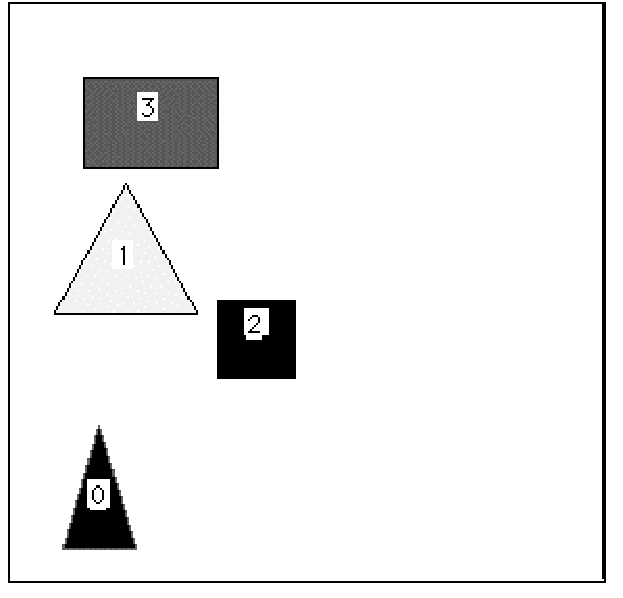
\includegraphics[width=.40\textwidth]{chap4/figs/game24}}
\caption{\label{scene4} The scene used in game 24.}
\end{figure}
The relevant data after sensor-scaling for the 
two sensory channels involved are shown in \tabref{tab:t-game24}. 
\begin{table}
\begin{center}
\begin{tabular}{| l | l | l | l |} \hline
{\it Object} & {\it HEIGHT} & {\it WIDTH} \\ \hline
0 (triangle) & 0.170 & 0.513  \\ \hline
1 (triangle) & 0.653 & 0.570 \\ \hline 
2 (square) & 0.213 & 0.213 \\ \hline 
3 (rectangle) & 0.613 & 0.310 \\ \hline 
\end{tabular}
\caption{\label{tab:t-game24} Sensory data for the scene in \figref{scene4}.}
\end{center}
\end{table}

[HEIGHT 0.0-0.5] is valid for triangle-0 and square-2 but
filters out the other segments. 
[WIDTH 0.5-1.0] is valid for triangle-0 and triangle-1 and 
filters out the others.  
The conjunctive combination of these two categories only 
retains triangle-0 and is therefore the one that is chosen. 

\subsection{A real world scene}

The next example is taken from a series of discrimination 
games played by physically instantiated agents using 
real world images. The series is discussed more extensively 
in chapter 7. The agent {\bf a2} has 
captured the image shown in \figref{f:plate-10}
(top left) and done the necessary segmentation and 
gathering of sensory characteristics. The resulting sensory
values (after sensor-scaling) for the segments are shown
in \tabref{tab:t-real}. Object-0 has been selected as the topic. 
\begin{table}
\begin{center}
\begin{tabular}{| l | l | l | l |} \hline
{\it channel}& {\it obj-0} & {\it obj-1} & Saliency\\ \hline
HPOS & 0.27 & 0.16 & 0.11\\ \hline
VPOS & 0.20 & 0.20 & 0.0\\ \hline
HEIGHT & 0.15 & 0.15 & 0.0\\ \hline
WIDTH & 0.10 & 0.11 & 0.01\\ \hline
AREA & 0.10 & 0.10 & 0.0\\ \hline
R & 0.23 & 0.25 & 0.02\\ \hline
G & 0.32 & 0.34  & 0.02\\ \hline
B & 0.63 & 0.65 & 0.02\\ \hline
\end{tabular}
\caption{\label{tab:t-real} Sensory data from a real world scene with segmentation shown in \ref{f:plate-10}.}
\end{center}
\end{table}
Clearly HPOS is the most salient channel and should be 
prefered by the agent. When performing context scaling, 
the two values for HPOS are drawn apart with 1.0 for object-0 and 
0.0 for object-1 so that the category [HPOS 0.5-1.0] (to the 
right) easily distinguishes the topic (object-0) from
object-1. The game is reported as follows: 
\begin{verbatim}
Game 3 
  a2 is the speaker. a1 is the hearer. 
  a2 segments the context into 2 objects: 
       object-0 object-1
  a2 chooses object-0 as the topic 
  a2 categorizes the topic as [HPOS 0.5-1.0]
\end{verbatim}
This example illustrates well why the categorization 
of the Talking Heads is so robust and why agents 
often share the same conceptualisation even if the details  
of their raw perception is quite different. 
The saliency factor helps to focus the agents on those
aspects of the scene that stand out. There is 
an enormous reduction of variation, first by scaling then by 
the categorization process itself. 

\section{An ecology of distinctions}

The previous section introduced mechanisms that 
enable agents to find a distinctive category or
conjunctive combination of categories given 
a set of segments and data on a series of sensory 
channels for each segment. I will now focus on the 
issue how discrimination networks and hence
repertoires of possible categories may develop. 

\subsection{Growth dynamics}

The process of growing categorizers is relatively
straightforward. In the very beginning, the agent
constructs top level categorizers for each channel which 
have contained at least once 
in the recent past relevant and distinctive
data. If a channel has the same data for every 
possible segment it is obviously not going to be 
possible to find a distinctive category no matter
how hard the agent tries. 

A new subcategorizer is constructed by taking a
categorizer node in the tree and dividing its range into 
two new subranges and thus two new subcategorizers.
For example, if there is a 
categorizer [HPOS 0.0-0.5], which triggers when the 
object is in the left most half of a scene, i.e. with HPOS
within $[0.0,0.5]$, then two 
subcategories are created by dividing $[0.0,0.5]$
into two halves, one for the 
range $[0.0,0.25]$ ([HPOS 0.0-0.25] or totally left) 
and one for the range $[0.25,0.5]$ ([HPOS 0.25-0.5] or mid-left). 
A new categorizer is added to the tree for each of these
halves. 

A categorizer based on a combination of categories is 
constructed by combining existing categories into a new one. 
Of course, if done without limits, this could create potentially 
a combinatorial explosion of possibilities. In the 
current implementation, the construction of combinations
is restricted by combining only those categories that 
have been partially successful in a given scene, 
just as only categories that
have ever been relevant are expanded. 

There are two key parameters to the growth process: 
(1) which category should be expanded and (2) when should
growth take place. In the Talking Heads experiment, agents expand 
a category which was effectively applied in the 
recent past, even though it may have failed in the game. 
This way the network is more likely to 
develop branches that are potentially relevant, although 
there is still no guarantee that the expansion
gives the distinctions required for the case at hand, 
because it is not based on an in-depth analysis of 
the case. 

Growth rate is proportional to failure. The more failures 
occur, the higher the likelihood of more nodes growing. This has the 
net effect of many new nodes growing in the beginning because
there are many failures, but that the repertoire of
categories stabilises
once discriminatory success is steady. When the environment 
starts to change again, causing new failures, more active 
growth is automatically triggered, which may lead 
to a renewed expansion of the repertoire. 

\subsection{Pruning dynamics}

Growth needs to be balanced by pruning. Pruning simply means
that a categorizer and thus its pending branches is 
cut away. There are again two
issues: (1) which nodes should be pruned and
(2) when pruning should take place. 
Obviously the score of a category should play a role
in deciding whether it should be pruned. 
categorizers that have not been used very much or have a low
success rate are prime candidates for removal, unless
any of their subcategorizers has a high score. The 
monitoring of use and success already played a role in 
determining which category should be prefered, so this
information is available to decide on pruning as well. 

Whereas the growth rate is proportional to failure, the pruning
rate is made proportional to success, so that 
in the case of a high failure rate the new categorizers are given
time to improve their score or to grow refinements that may be 
successful. A new categorizer obviously should be given
a grace period to encounter enough cases to prove
its worth, otherwise it could be cut out too quickly. Categorizers 
therefore not only monitor their use and success but 
also their age. 

\subsection{Average discriminatory success and repertoire size}

\is{discriminatory success}The Discrimination Game is a dynamical system.\footnote{
The theory of complex dynamical systems, which is well 
developed in the natural sciences, provides the 
theoretical foundation for studying the Discrimination
Game. For a general introduction, see \cite{Peitgen:1992}. 
Applications of these techniques to study the origins
of complexity based on computer simulations 
can be found in the regular conferences on Artificial
Life, proceedings published by MIT Press, Cambridge Ma.} A repertoire of
categories emerges in an agent gradually as an attractor of the
growth and pruning dynamics coupled to 
the environment. If growth is strictly proportional to failure
and there is no pruning, a point attractor
is reached as soon as the repertoire
is adequate, i.e. as soon 
as the agent consistently has success
for all the possible cases it encountered. However, 
as soon as the environment or the sensory capabilities of 
the agent change, in other words when new types of 
figures appear or when new sensory channels become available
to the agent, we expect that the repertoire of categories starts
expanding again. This could be seen as an illustration  of the
assimilation-accomodation dynamics envisioned by Piaget. 

Let me introduce a few measures 
to test whether all this is really happening with the 
mechanisms introduced so far.
The first (crucial) measure monitors 
how well the agent is doing by tracking
the average success in the most recent $n$ discrimination games. 
\figref{avsuc} shows the outcome of this measure, for 
agent {\bf a1}, playing 500 discrimination games in a
simulation with scenes from the GEOM world. 
Success is averaged per 25 games. We see clearly that {\bf a1}
has become successful in discriminating randomly chosen topics
from a consecutive series of scenes. Success rapidly climbs and
reaches 100 \%, even though the scenes are randomly
generated combinations from a repertoire of figures
along continuously varying 
dimensions making for literally billions of possibilities. 
The Discrimination Game is successful because it does 
not try to detect invariants or commonalities between consecutive 
cases but focuses on finding what is distinctive between the topic 
and the other objects. This enables the agent to make
such a gigantic abstraction leap and to make it at an amazingly 
rapid speed. 
\begin{figure}[htbp]
  \centerline{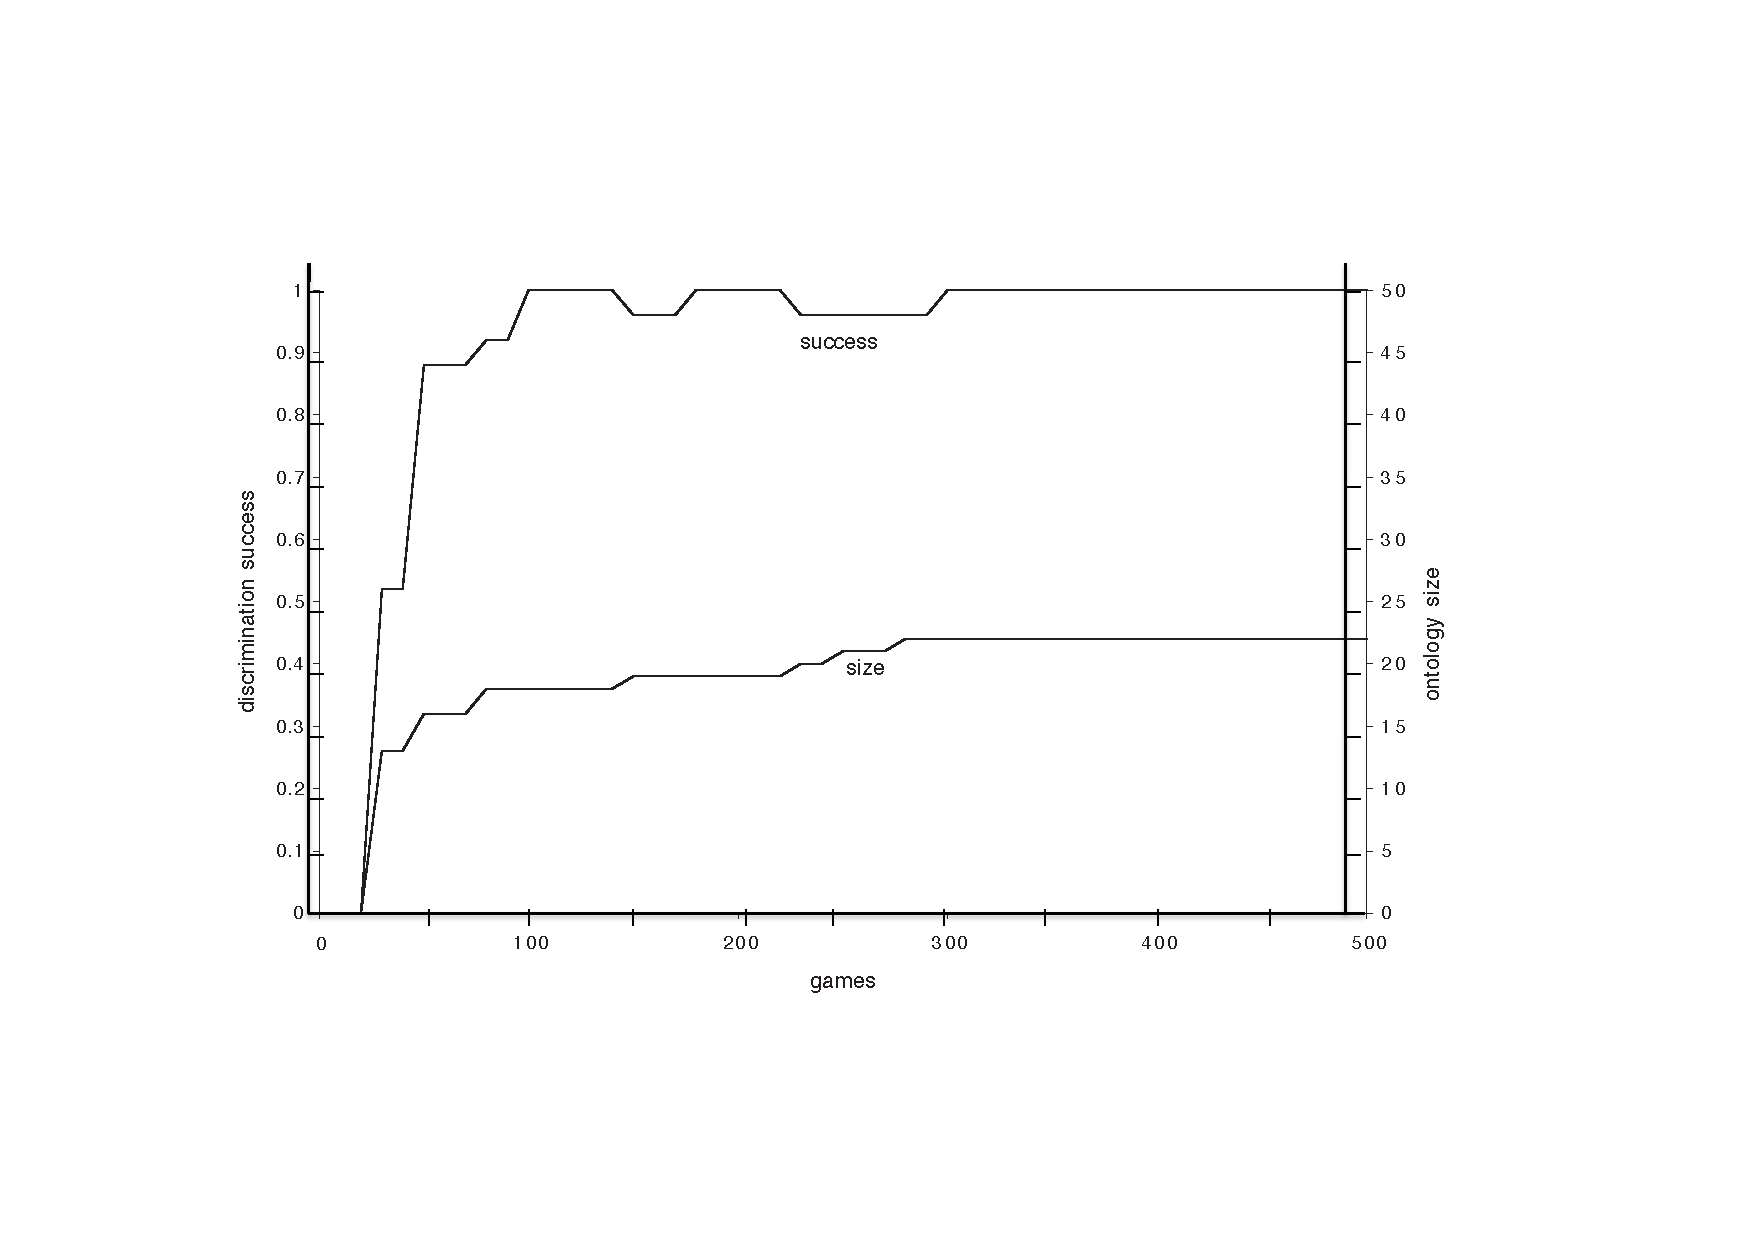
\includegraphics[width=.70\textwidth]{chap4/figs/avsuc}}
\caption{\label{avsuc} The graph displays the 
average success per 25 discrimination games for a
series of 500 games played by a single agent. Success climbs
to 100 \%. The graph also displays the size of the 
agent's repertoire of categories. Each scene contains
between 3 and 6 objects.}
\end{figure}

We can see whether a stable attractor has been reached by 
tracking the size of the repertoire, which is
simply the number of 
categorizers in the agent's discrimination trees. 
The result of this measure is also displayed in 
\figref{avsuc}. Once success is steady, the
size of the repertoire remains 
constant, which means that no new 
elementary distinctions arise nor do any distinctions
disappear. This is because there has been no pruning yet and 
growth is strictly proportional to failure. 

\figref{dyna-trees} shows some snapshots of the 
evolution in the discrimination trees of {\bf a1} as
the simulation continues and as additional situations
arise. There are
expansions, contractions, and shifts in the constitution of the 
discrimination trees but gradually there are fewer and 
fewer changes (compare for example (c) and (d)) as a
stable core emerges. 
\begin{figure}[htbp]
  \centerline{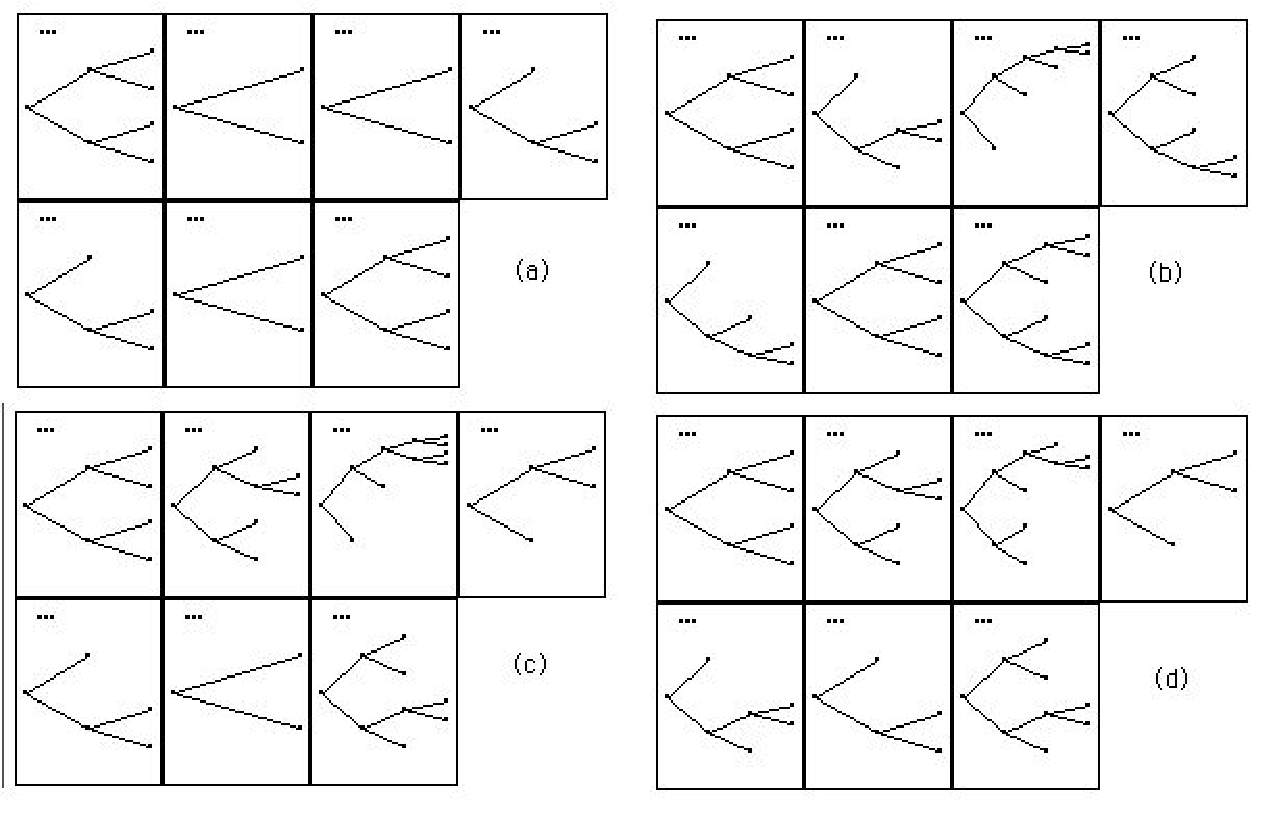
\includegraphics[width=.75\textwidth]{chap4/figs/dynatrees}}
\caption{\label{dyna-trees} Some snapshots of an evolving 
repertoire in a single agent using growth and pruning. 
Trees are shown after 500 games (a), 1000 games (b), 1500 games
(c) and 2000 games (d).} 
\end{figure}

These simulations show that the
category formation process based on a growth and pruning
dynamics is capable of creating a repertoire of
discrimination trees adequate for distinguishing 
the topic from other objects in the scene. The simulations 
worked with computer-generated, stylised environments
so that it is possible to probe the behavior of 
the mechanisms and vary the complexity of the environment. 
Note that the mechanisms are neutral with respect 
to the type of channels supplied. The discrimination 
trees and growth and pruning dynamics can operate over
auditory or bodily sensory channels, or other kinds
of visual information that is produced by low level 
perception. 

\subsection{Adaptivity in categorization}

\is{categorial adaptivity}An agent operating in a real world environment is always
going to be confronted with situations that he has 
not seen before. The growth and pruning dynamics of the 
discrimination game is capable of dealing with this because 
new distinctions grow when the failure rate 
is increasing. Here are the results of a computer 
simulation based on scenes generated by the 
GEOM world that test whether this is indeed the case. 

The simulation starts with a new virgin agent 
playing a series of discrimination games involving scenes
which only contain rectangles of the same graylevel. 
The agent has only channels for HEIGHT (0), WIDTH (1), 
RATIO (between the actual area of the shape 
and the area of the bounding box),
(2), GRAY (3) and AREA (4). We expect
to see that the discrimination trees on the RATIO (channel 
2) and GRAY channels (channel 3) do not develop because 
the values on those channels 
are the same for all objects ever seen. This is 
clearly confirmed in \figref{adptwrl1}: The ratio
between actual area and bounding box area is always 1.0
in the case of rectangles and they always have the same
grayscale value. 
We see clearly that the RATIO (channel 2) and GRAY (channel 3) 
do not develop and that the others develop to very 
fine levels of detail to still successfully discriminate. 
So discrimination trees only 
develop as needed in a particular environment, which is 
important for applying the selectionist
principle to the generation of sensory channels. 
The categorization process gives feedback to 
the sensory processing on the adequacy of particular sensory 
channels. 
\begin{figure}[htbp]
  \centerline{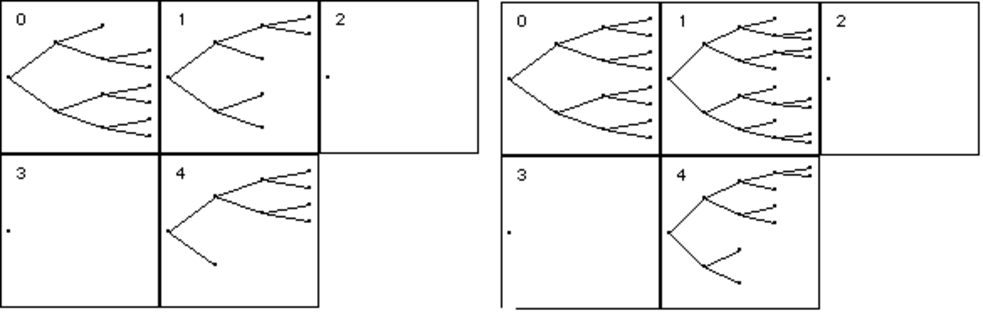
\includegraphics[width=.65\textwidth]{chap4/figs/adptwrl1}}
\caption{\label{adptwrl1} Two snapshots 
from a series of 500 discrimination 
games developing categories to distinguish rectangles of 
the same average graylevel. Channel 2 (the ratio channel) 
and channel 3 (the grayscale channel) do not develop.}
\end{figure}

Let us now make the environment richer by letting the 
GEOM world also produce scenes with circles and triangles, 
as well as rectangles. If the discrimination 
process is adaptive, the RATIO and GRAY channels should
start to expand because these channels now contain
significant data. This is indeed the case as shown 
in \figref{adptwrl2}. 
\begin{figure}[htbp]
  \centerline{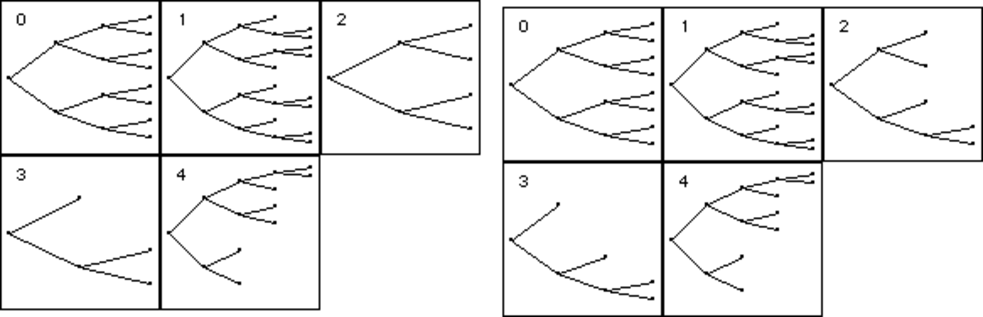
\includegraphics[width=.65\textwidth]{chap4/figs/adptwrl2}}
\caption{\label{adptwrl2} Two snapshots from 
an additional series of 500 discrimination games after
the environment has become more complex. RATIO
(channel 2) and GRAY (channel 3) have started to develop.}
\end{figure}

The simulation demonstrates
that the proposed discrimination process is adaptive to
changes in the environment, because growth picks up
as soon as the environment poses new challenges, just 
like the immune system starts generating a larger 
repertoire (and expanding already existing antibodies
that partially matched)
when challenged by the invastion of foreign bodies. 
The adaptation can be tracked with the success and 
repertoire size measures introduced earlier. 
When these measures are collected for the above example
(see \figref{adptwrlglo}), phase one shows clearly that 
when only rectangles are present, a stable 
repertoire gradually develops and that the success rate reaches 100 \%
after about 500 games. In phase two, when other types of 
shapes have been introduced,
the discrimination trees begin to expand again, now exploiting the
RATIO and GRAY channels to cope with the new types of objects.
Existing categories will of course still be adequate for 
many cases. After 500 more games, a new equilibrium
is reached. Steady discrimination success is seen with an 
enlarged repertoire.
\begin{figure}[htbp]
  \centerline{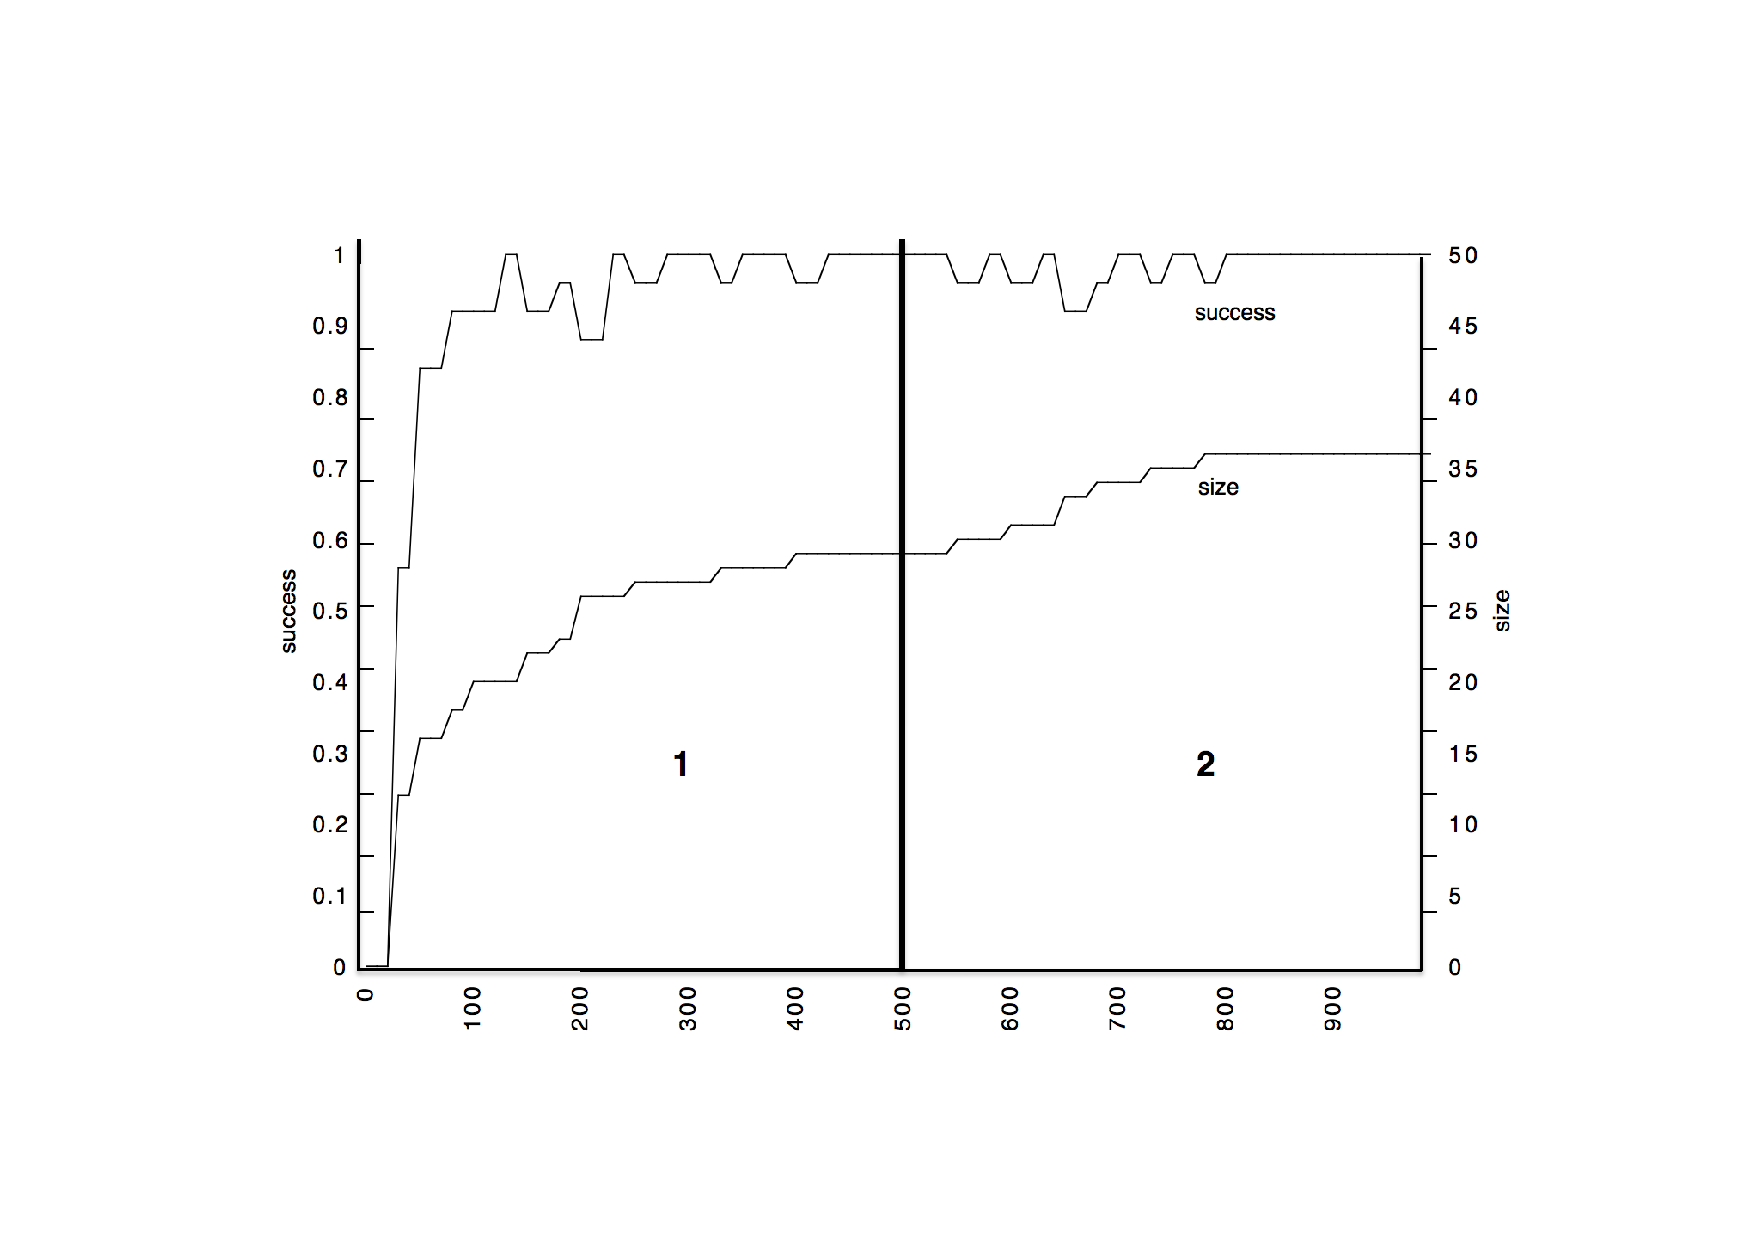
\includegraphics[width=.65\textwidth]{chap4/figs/adptwrlglo}}
\caption{\label{adptwrlglo} Evolution of success and ontology
size in a series of 1000 discrimination games played by a single agent.
In phase 1, only rectangles of the same graylevel are 
generated by the GEOM world. In phase 2, additional types of 
shapes are generated by the environment.}
\end{figure}

\subsection{Real world scenes}

Very similar developments can be seen when we do 
experiments with embodied agents, capturing real world scenes
through their cameras. \figref{discri200a} 
shows two snapshots of developing discrimination trees
for two agents. The game discussed earlier (based on 
plate 10, top) has been played with these trees. 
HPOS is the most salient channel and a distinction can 
be made easily. Note that the HEIGHT and WIDTH channels have not 
developed yet because no clear cases emerged 
in the environment where those channels provided 
salient data. 
\begin{figure}[htbp]
  \centerline{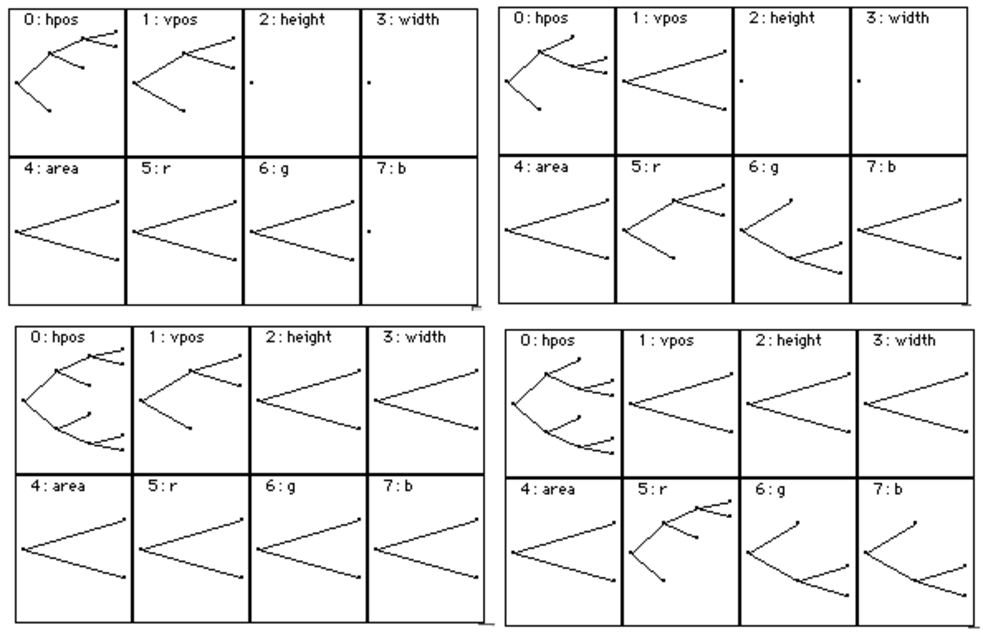
\includegraphics[width=.65\textwidth]{chap4/figs/discri200}}
\caption{\label{discri200a} The discrimination trees 
developed by two physically embodied agents 
{\bf a1} (left) and {\bf a2} (right). The top of the 
figure shows the trees after 
playing 100 games and bottom after 200 games.}
\end{figure}

\section{Conclusions}

This chapter addressed the problem of how agents may 
categorize their environment using information 
on sensory channels about each segment in the scene. 
I argued in favor of a selectionist approach, which 
generates possible solutions in a relatively 
random growth process and tests them in the 
cases presented by the environment. 
This approach contrasts with instructionism, where
the agent is assumed to make gradual abstraction 
from a series of examples using induction, and with 
a rationalist approach, where perceptually grounded categories are
assumed to be innate and hence derived through 
genetic evolution. 

The main conclusion of this chapter is that a selectionist
approach to the origins of categories
is theoretically and practically feasable. I have 
defined a growth and pruning dynamics which leads to 
an adequate repertoire for 
discriminating one object from the others in the 
same context and I showed that the repertoire is
continuously adapted when the environment changes. 

We will have plenty of opportunity in later chapters
to further test the mechanisms for categorization 
presented here. I will also introduce 
additional feedback couplings from the lexical 
layer to these categorization processes. Nevertheless
we are now sufficiently advanced to be able to
turn to the next subtask the agents face when 
engaging in a language game: establishing a relation
between categories or combinations of categories and 
an utterance. 

%There has been a long tradition of arguments for and 
%against a tight interaction between language and meaning, 
%exemplified with the debate triggered by the writings of 
%Whorf (See: \cite{Lee:1996} A recent survey of opinion and evidence
%can be found in: \cite{Gumperz:1996}.}

